% Options for packages loaded elsewhere
\PassOptionsToPackage{unicode}{hyperref}
\PassOptionsToPackage{hyphens}{url}
%
\documentclass[
]{article}
\usepackage{amsmath,amssymb}
\usepackage{iftex}
\ifPDFTeX
  \usepackage[T1]{fontenc}
  \usepackage[utf8]{inputenc}
  \usepackage{textcomp} % provide euro and other symbols
\else % if luatex or xetex
  \usepackage{unicode-math} % this also loads fontspec
  \defaultfontfeatures{Scale=MatchLowercase}
  \defaultfontfeatures[\rmfamily]{Ligatures=TeX,Scale=1}
\fi
\usepackage{lmodern}
\ifPDFTeX\else
  % xetex/luatex font selection
\fi
% Use upquote if available, for straight quotes in verbatim environments
\IfFileExists{upquote.sty}{\usepackage{upquote}}{}
\IfFileExists{microtype.sty}{% use microtype if available
  \usepackage[]{microtype}
  \UseMicrotypeSet[protrusion]{basicmath} % disable protrusion for tt fonts
}{}
\makeatletter
\@ifundefined{KOMAClassName}{% if non-KOMA class
  \IfFileExists{parskip.sty}{%
    \usepackage{parskip}
  }{% else
    \setlength{\parindent}{0pt}
    \setlength{\parskip}{6pt plus 2pt minus 1pt}}
}{% if KOMA class
  \KOMAoptions{parskip=half}}
\makeatother
\usepackage{xcolor}
\usepackage{graphicx}
\makeatletter
\def\maxwidth{\ifdim\Gin@nat@width>\linewidth\linewidth\else\Gin@nat@width\fi}
\def\maxheight{\ifdim\Gin@nat@height>\textheight\textheight\else\Gin@nat@height\fi}
\makeatother
% Scale images if necessary, so that they will not overflow the page
% margins by default, and it is still possible to overwrite the defaults
% using explicit options in \includegraphics[width, height, ...]{}
\setkeys{Gin}{width=\maxwidth,height=\maxheight,keepaspectratio}
% Set default figure placement to htbp
\makeatletter
\def\fps@figure{htbp}
\makeatother
\setlength{\emergencystretch}{3em} % prevent overfull lines
\providecommand{\tightlist}{%
  \setlength{\itemsep}{0pt}\setlength{\parskip}{0pt}}
\setcounter{secnumdepth}{-\maxdimen} % remove section numbering
\ifLuaTeX
  \usepackage{selnolig}  % disable illegal ligatures
\fi
\IfFileExists{bookmark.sty}{\usepackage{bookmark}}{\usepackage{hyperref}}
\IfFileExists{xurl.sty}{\usepackage{xurl}}{} % add URL line breaks if available
\urlstyle{same}
\hypersetup{
  pdftitle={Operating\_System\_(OS)},
  hidelinks,
  pdfcreator={LaTeX via pandoc}}

\title{Operating\_System\_(OS)}
\author{}
\date{}

\begin{document}
\maketitle

\hypertarget{what-is-an-os}{%
\section{What is an OS}\label{what-is-an-os}}

An OS is a \textbf{layer of software} that \textbf{interfaces} between
hardware ressources and one or multiple applications running on the
machine. It is a special program that should \textbf{never stop} and
\textbf{never fail}. It is fully \textbf{trusted} by hardware and
applications.

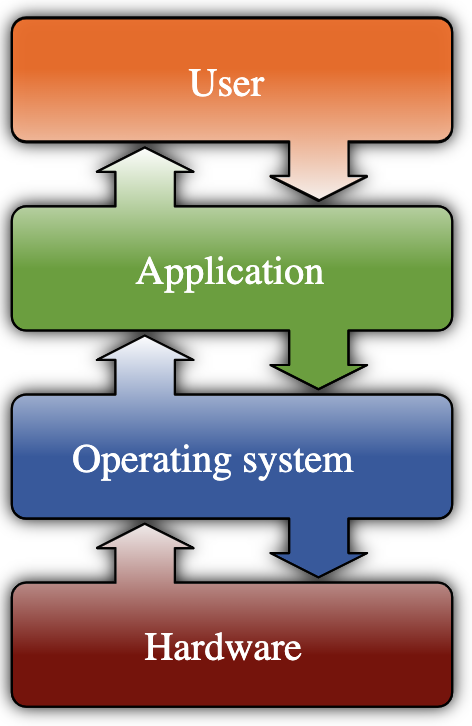
\includegraphics[width=1.5625in,height=\textheight]{/home/noaemien/Desktop/Personal/mindhive/Pasted_image_20240312210618.png}

\hypertarget{the-os-provides}{%
\subsection{The OS Provides}\label{the-os-provides}}

\hypertarget{protection-isolation-and-sharing-of-resources}{%
\subsubsection{\texorpdfstring{\textbf{Protection}, \textbf{isolation}
and sharing of
resources}{Protection, isolation and sharing of resources}}\label{protection-isolation-and-sharing-of-resources}}

\hypertarget{fault-isolation}{%
\paragraph{Fault isolation}\label{fault-isolation}}

Fault isolation is intended to separate Processes from each-other as
well as from the OS\\
Un-allowed access results in \textbf{Segmentation fault}

\hypertarget{ressource-sharing}{%
\paragraph{Ressource sharing}\label{ressource-sharing}}

Scheduling\\
The OS needs to choose which process to execute, as well as how much of
each physical ressource to allocate to each process.

\hypertarget{communication}{%
\paragraph{Communication}\label{communication}}

The OS allows processes to communicate with each other in a protected
manner

\hypertarget{clean-and-easy-to-use-abstraction-of-physical-ressources}{%
\subsubsection{\texorpdfstring{Clean and easy to use \textbf{abstraction
of physical
ressources}}{Clean and easy to use abstraction of physical ressources}}\label{clean-and-easy-to-use-abstraction-of-physical-ressources}}

\textbf{Virtualization} is used to give applications the illusion of
exclusive CPU access along with the illusion of infinite hardware
ressources.

Higher level objects such as files, users and messages are used.

\hypertarget{process-abstraction}{%
\paragraph{Process Abstraction}\label{process-abstraction}}

The OS provides process abstraction to every program, enabling each
process to execute in a restricted execution environment

Processes have a nicer interface than raw hardware: Threads, Address
space, Files and Sockets\\
The OS translates from hardware interface to application interface.\\
It provides each running program with its own process.\\
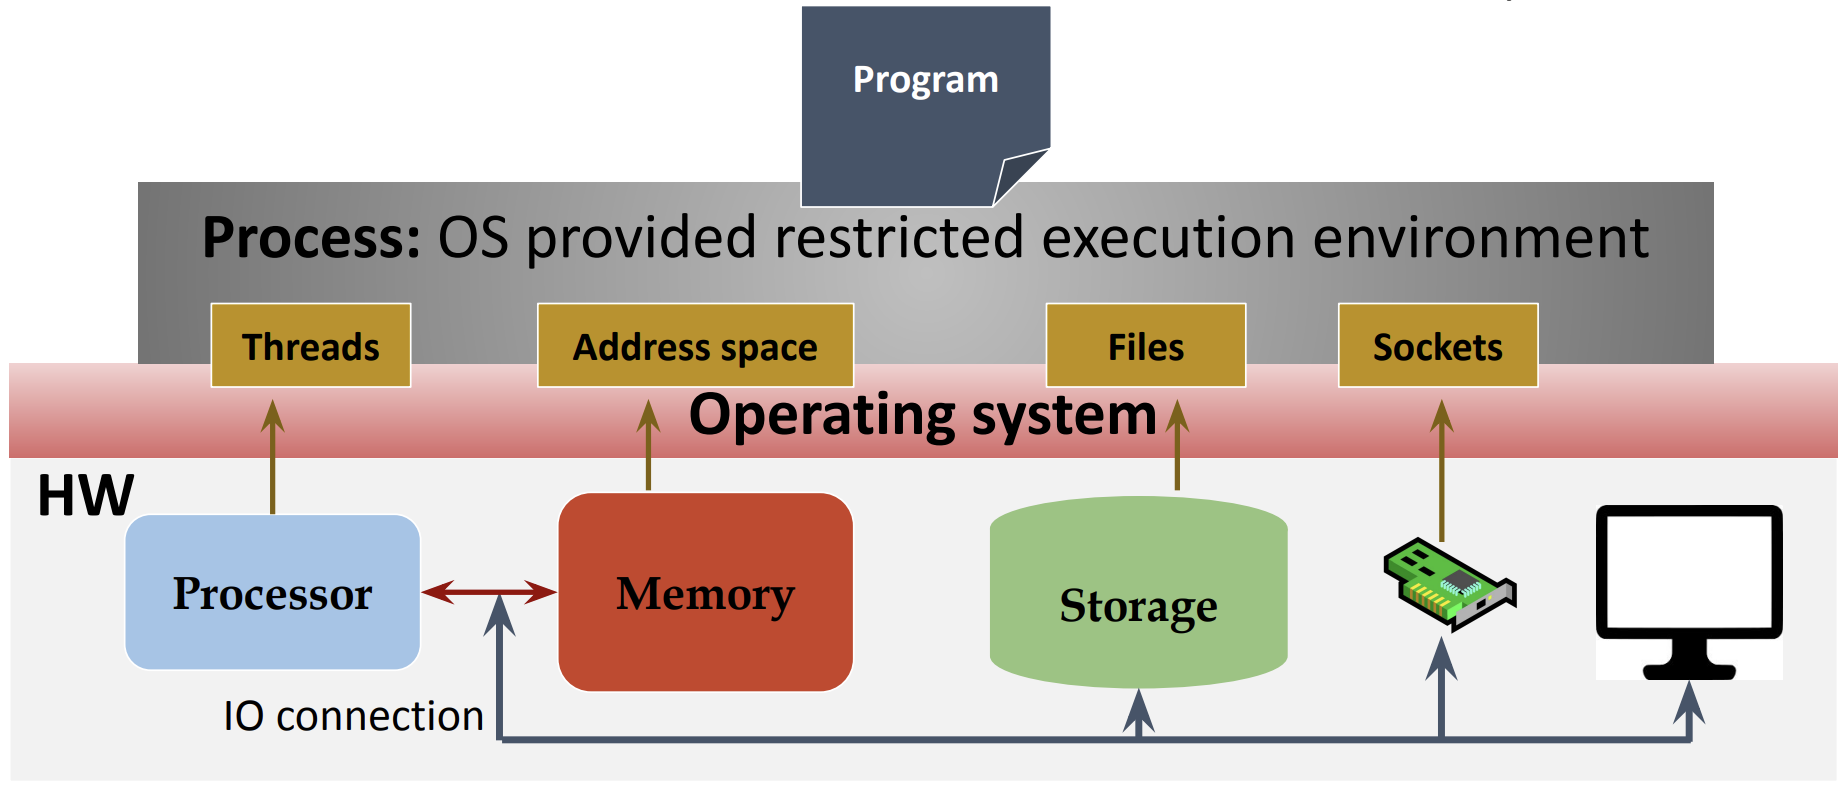
\includegraphics{/home/noaemien/Desktop/Personal/mindhive/Pasted_image_20240312211634.png}

\hypertarget{a-set-of-common-services}{%
\subsubsection{\texorpdfstring{A set of \textbf{common
services}}{A set of common services}}\label{a-set-of-common-services}}

The OS provides a set of common services to standardise the design of
applications.\\
This makes sharing easier and maximises reuse as all applications are
built upon the same base.\\
Decouples application development from hardware.

For example:

\begin{itemize}
\tightlist
\item
  File Systems
\item
  User Interface
\item
  Network
\end{itemize}

\hypertarget{how-os-handles-processes}{%
\section{How OS handles processes}\label{how-os-handles-processes}}

The OS keeps a tree of all processes

\begin{itemize}
\tightlist
\item
  Every process has a parent except "init" (pid 1 = init)
\item
  The OS Scheduler maintains the set of schedulable processes
\end{itemize}

\hypertarget{running-a-process}{%
\subsection{Running a process}\label{running-a-process}}

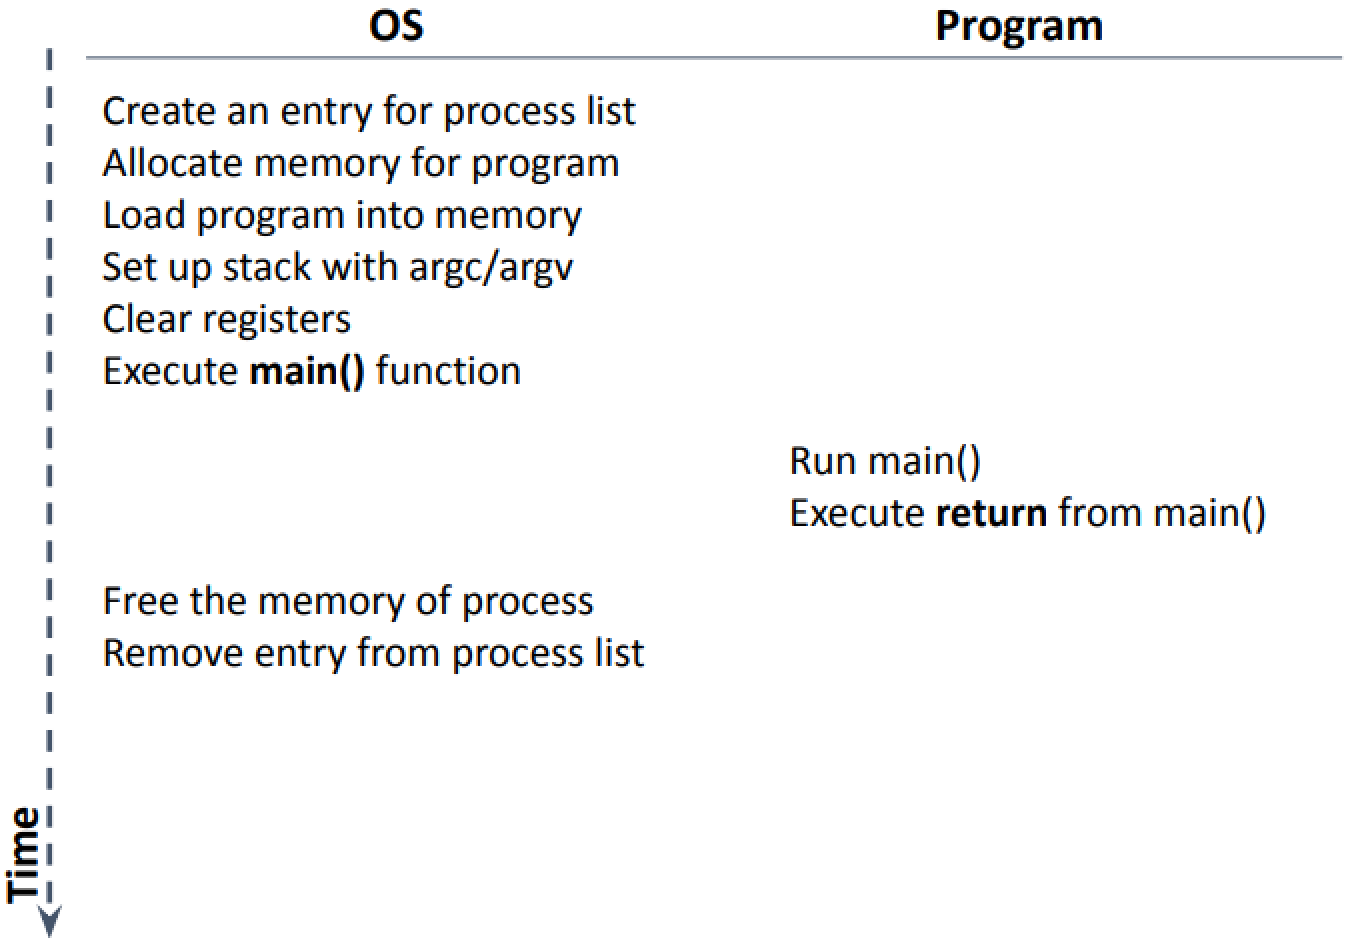
\includegraphics[width=5.20833in,height=\textheight]{/home/noaemien/Desktop/Personal/mindhive/Pasted_image_20240318141157.png}

\hypertarget{keeping-control-interrupts}{%
\subsection{Keeping Control:
Interrupts}\label{keeping-control-interrupts}}

\begin{itemize}
\tightlist
\item
  provided by hardware as a signaling mechanism for OS~to maintain
  Control
\item
  \textbf{Asynchronous}, signals some external event has happened and
  needs attention
\item
  Interrupts are disabled when an interrupt handler is running
\end{itemize}

\hypertarget{handling}{%
\paragraph{Handling}\label{handling}}

\begin{itemize}
\tightlist
\item
  Detected by CPU
\item
  Suspends running process
\item
  Executes interrupt handling code in kernel mode
\item
  Restores the user process\\
  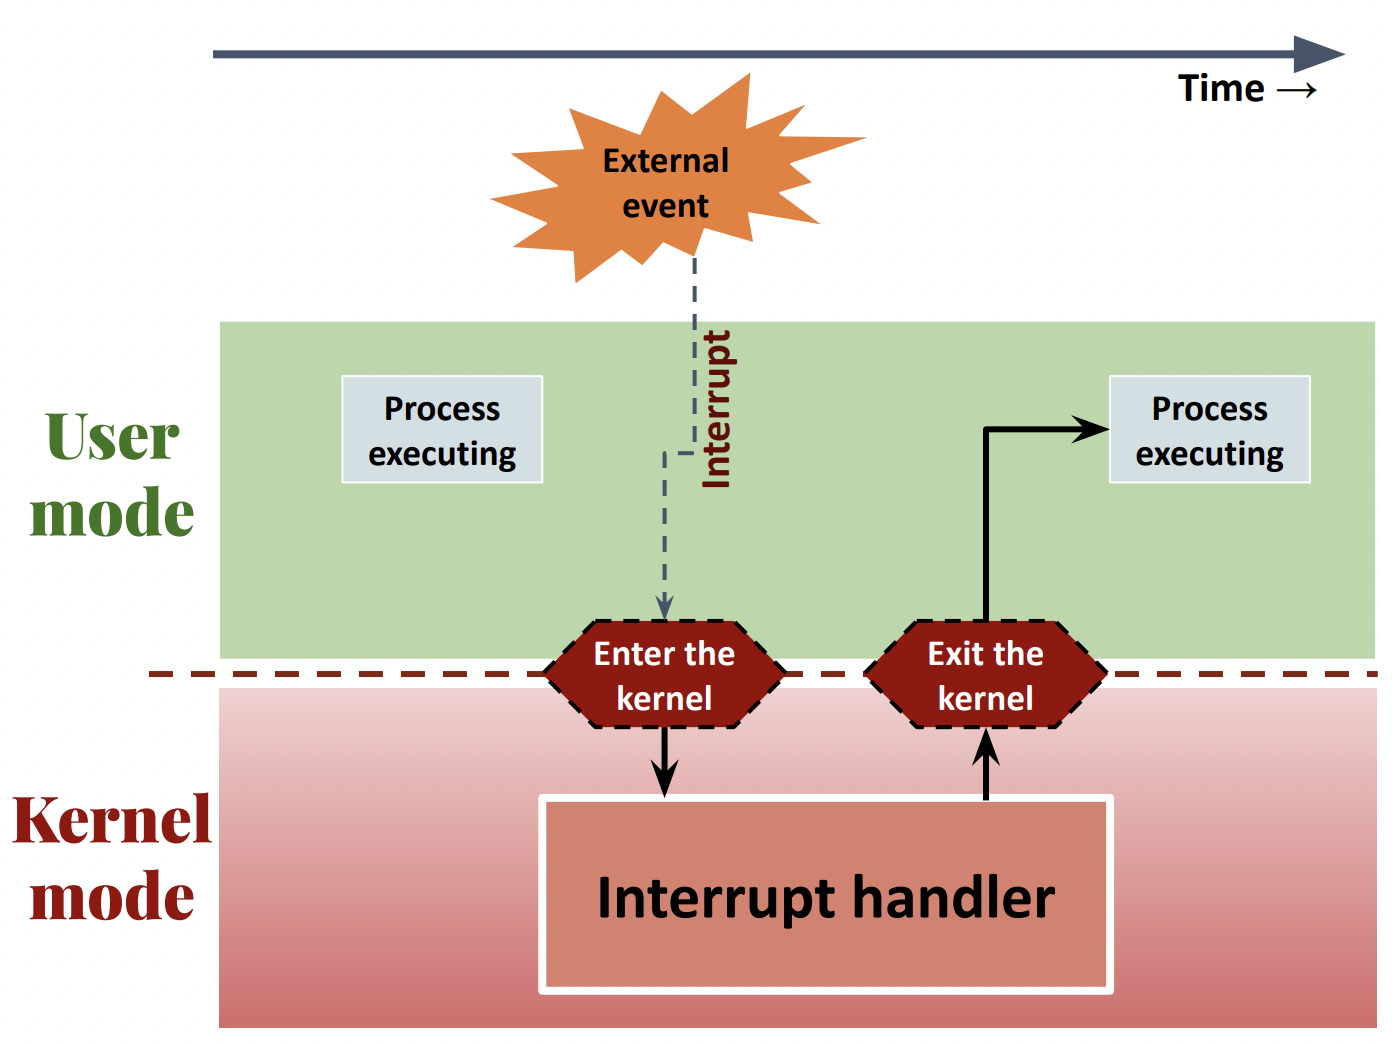
\includegraphics[width=5.20833in,height=\textheight]{/home/noaemien/Desktop/Personal/mindhive/InterruptHandling.png}
\end{itemize}

\hypertarget{example}{%
\subsubsection{Example}\label{example}}

\textbf{Timer Interrupt}:~Interrupts every 10 ms for OS to regain
control

\begin{itemize}
\tightlist
\item
  Every 10 ms CPU switches from user to kernel mode
\item
  Now OS can choose which process to execute
\end{itemize}

\hypertarget{scheduling}{%
\subsection{Scheduling}\label{scheduling}}

\hypertarget{mechanism}{%
\subsubsection{Mechanism}\label{mechanism}}

\hypertarget{context-switch}{%
\paragraph{Context Switch}\label{context-switch}}

The act of stopping one process and running an other one\\
Happens the OS~is in kernel mode and:

\begin{itemize}
\tightlist
\item
  Cannot return to the same process

  \begin{itemize}
  \tightlist
  \item
    Process has terminated
  \item
    Process is waiting on I/O
  \end{itemize}
\item
  Does not want to return to same process

  \begin{itemize}
  \tightlist
  \item
    Process has run for too long
  \item
    Other processes are present and need to be scheduled
  \end{itemize}
\end{itemize}

\hypertarget{procedure}{%
\subparagraph{Procedure}\label{procedure}}

Context of process is maintained in Process Control Block (PCB)\\
OS maintains process control block for each process\\
PCB contains:

\begin{itemize}
\tightlist
\item
  All process specific registers
\item
  All general registers\\
  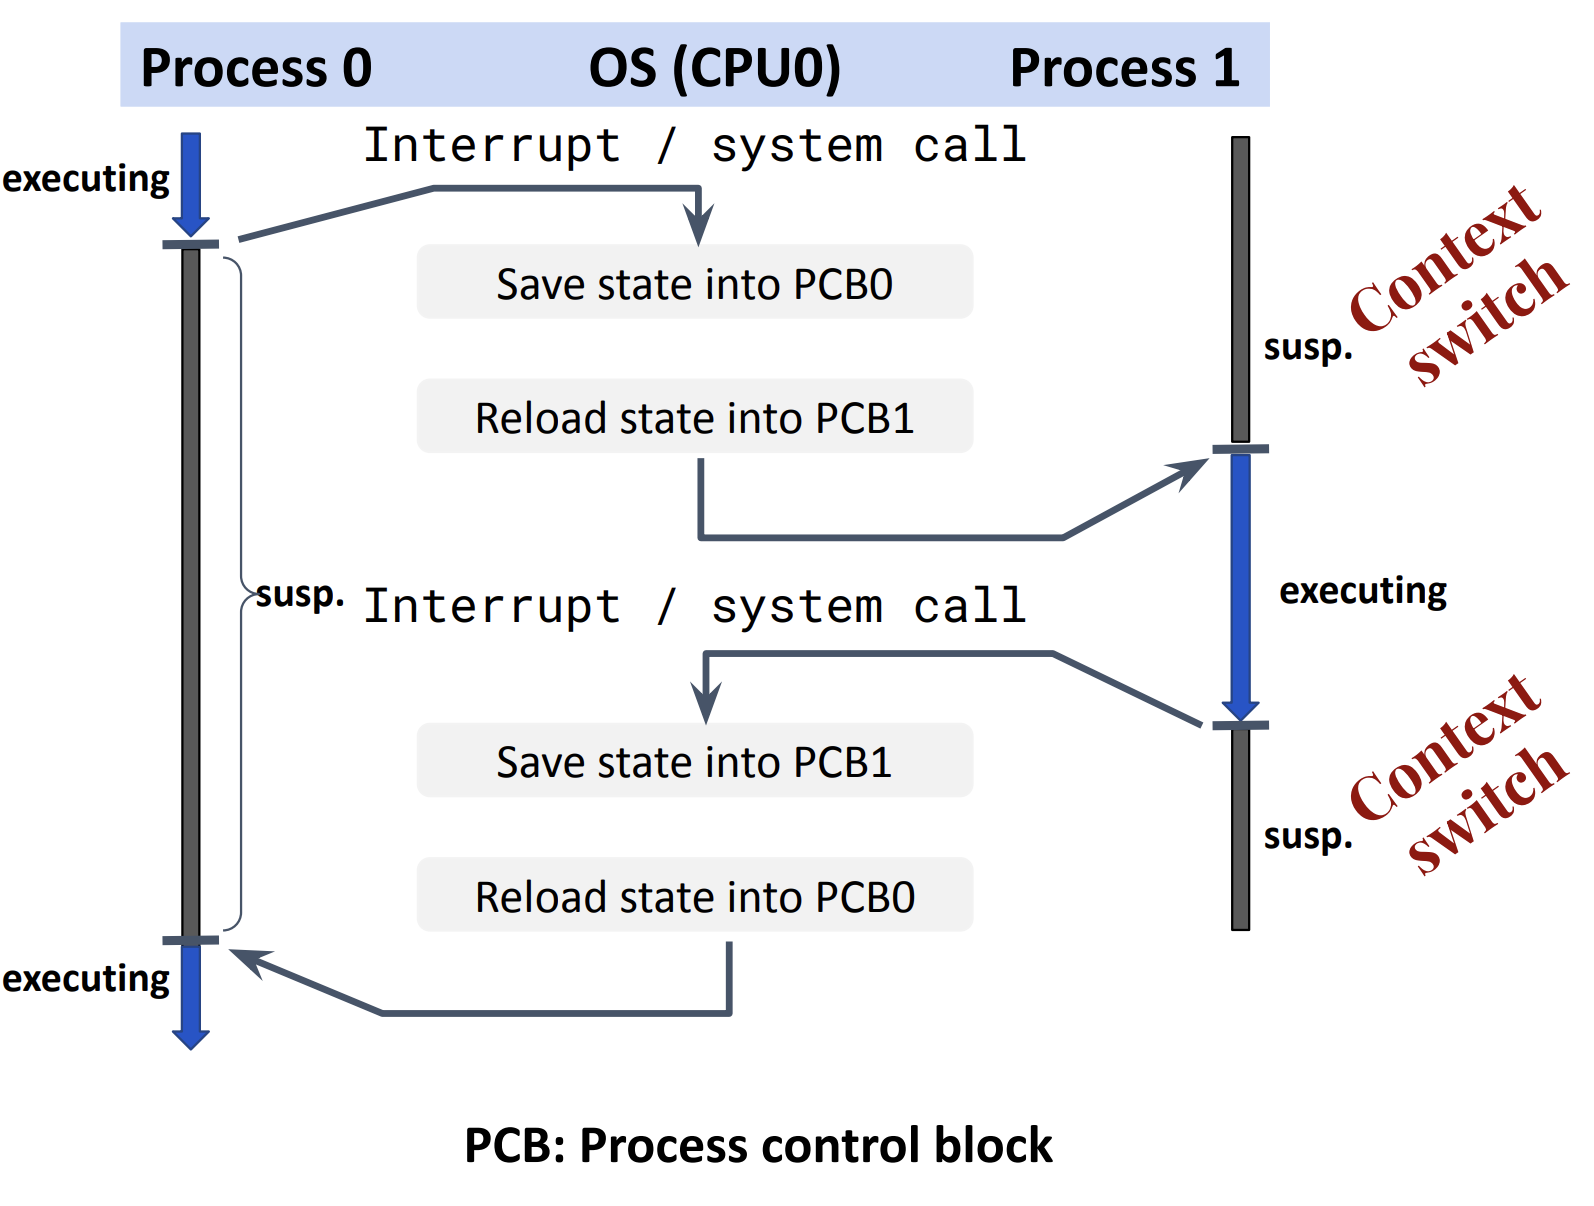
\includegraphics[width=4.16667in,height=\textheight]{/home/noaemien/Desktop/Personal/mindhive/contextSwitchProcedure.png}\\
  De-scheduled process is either is \textbf{Ready} or \textbf{Blocked}
  state
\end{itemize}

\hypertarget{preemption}{%
\subsubsection{Preemption}\label{preemption}}

OS sets a timer before scheduling a process to avoid process running for
ever

\begin{itemize}
\tightlist
\item
  Hardware sends interrupt after timer expires
\item
  Interrupts process execution
\item
  Switch to kernel mode
\item
  OS~decides if process can continue or if it performs a context switch
\end{itemize}

\hypertarget{metrics}{%
\subsubsection{Metrics}\label{metrics}}

\hypertarget{utilization}{%
\paragraph{Utilization}\label{utilization}}

Fraction of the time CPU~is executing a job\\
\textbf{Goal:} Maximize CPU utilization

\hypertarget{turnaround-time}{%
\paragraph{Turnaround Time}\label{turnaround-time}}

Total time from job arrival to job completion\\
\textbf{Goal:} Minimize turnaround time

\hypertarget{response-time}{%
\paragraph{Response Time}\label{response-time}}

Total time from job arrival until first time job is scheduled

\hypertarget{policies}{%
\subsubsection{Policies}\label{policies}}

\hypertarget{non-preemptive}{%
\paragraph{Non preemptive}\label{non-preemptive}}

\hypertarget{fifo-first-in-first-out}{%
\subparagraph{FIFO (First in First Out)}\label{fifo-first-in-first-out}}

Complete jobs in chronological orders of arrival\\
Suffers from Convoy effect

Convoy effect

Short jobs get queued behind a long job that arrived first.

\hypertarget{sjf-shortest-job-first}{%
\subparagraph{SJF (Shortest Job First)}\label{sjf-shortest-job-first}}

Execute shortest job first assuming they arrive at the same time,
otherwise execute first arrived

\textbf{Long running jobs cannot be interrupted for shorter jobs that
arrive after}

\hypertarget{preemptive}{%
\paragraph{Preemptive}\label{preemptive}}

\hypertarget{stcf-shortest-time-to-completion-first}{%
\subparagraph{STCF (Shortest Time to Completion
First)}\label{stcf-shortest-time-to-completion-first}}

Extends SJF by adding preemption.\\
Each time a new job enters the system:

\begin{itemize}
\tightlist
\item
  Scheduler determines which of remaining jobs has shortest completion
  time
\item
  Schedules the shortest job first
\end{itemize}

\textbf{Not great response time}

\hypertarget{rr-round-robin}{%
\subparagraph{RR (Round-Robin)}\label{rr-round-robin}}

Runs jobs for fixed time-slice and the switches to next job

\hypertarget{taking-io-into-account}{%
\paragraph{Taking I/O into account}\label{taking-io-into-account}}

I/O is generally slow so scheduler should schedule other jobs during I/O

\hypertarget{multi-level-feedback-queue-mlfq}{%
\subparagraph{Multi-Level Feedback Queue
(MLFQ)}\label{multi-level-feedback-queue-mlfq}}

\textbf{Goal:} General Purpose Scheduler\\
\textbf{Challenge:} Supporting long running, CPU intensive jobs (Batch
processing) and interactive, low latency foreground tasks (interactive
processes)

First \emph{optimizes} average turnaround time

\begin{itemize}
\tightlist
\item
  Important for batch processes\\
  Then \emph{minimizes} response time
\item
  Important for interactive processes
\end{itemize}

\hypertarget{approach-multiple-levels-of-round-robin}{%
\subparagraph{Approach:~Multiple levels of Round
Robin}\label{approach-multiple-levels-of-round-robin}}

Each level has higher priority and preempts lower level\\
Process at a higher level will always be scheduled first\\
High levels have short time slices, lower levels run longer

Rule 1: if priority(A) \textgreater{} priority(B) then A runs\\
Rule 2: if priority(A) == priority(B) then A \& B run in RR\\
Rule 3: Processes start at top priority\\
Rule 4: If a process uses its total time slice, the scheduler lowers its
priority\\
Rule 5: Periodically moves all jobs to topmost queue (\textbf{priority
boosting})

Boosting avoids starvation (long tasks never being scheduled1)

\hypertarget{idle-process}{%
\paragraph{Idle process}\label{idle-process}}

Process that runs if all processes are blocked\\
Has low priority\\
Never blocks or does I/O

\end{document}
